\documentclass[
    oneside,
    ngerman,
    footinclude=false,
    captions=tableheading,
    DIV=12
]{scrartcl}


\usepackage{UniLaTeXPackage}

\ihead{Tom Folgmann,\\David Jannack}
\chead{TUTOR\\Blattsammlung}
\ohead{\today}

\begin{document}
    \aufgabe{}
        \subaufgabe{}
            \paragraph*{Lösung mit Euler (explizit)}
                Die folgenden Graphen zeigen die numerische Entwicklung von Ort und Geschwindigkeit.
                \begin{figure}[H]
                    \centering
                    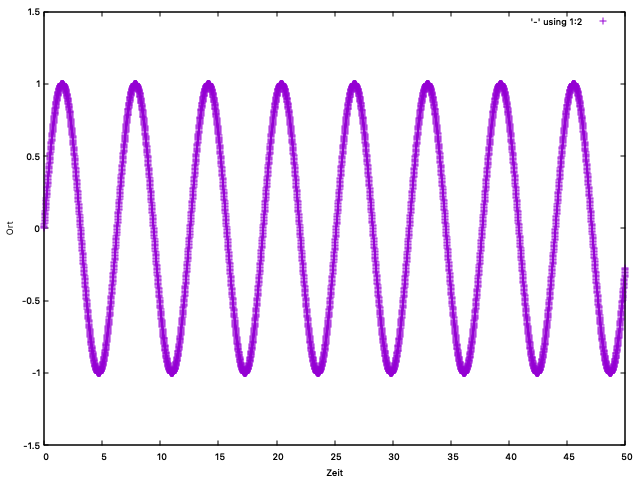
\includegraphics[width=8cm]{Bilddateien/expEulerA1(a)-001h-x.png}
                    \caption{Ortsdiagramm}
                \end{figure}
                \begin{figure}[H]
                    \centering
                    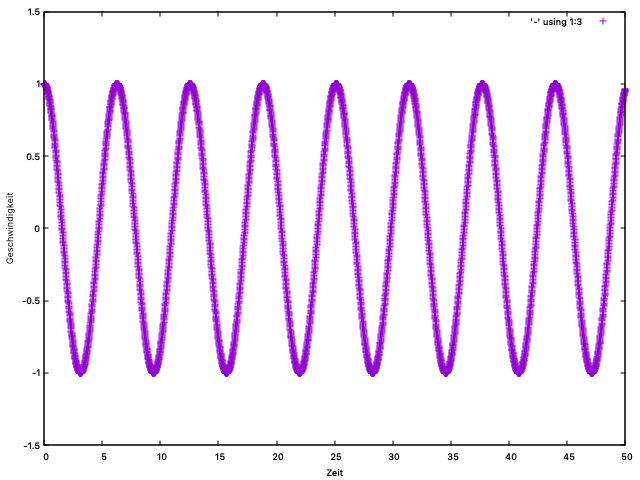
\includegraphics[width=8cm]{Bilddateien/expEulerA1(a)-001h-v.png}
                    \caption{Geschwindigkeitsdiagramm}
                \end{figure}
                Man sieht klar den zu erwarteten sinusförmigen und zueianander phasenverschobenen Verlauf beider Größen. Die Amplitde bleibt ebenso im Zuspruch mit der exakten Lösung konstant. Das folgende Diagramm stellt nochmal die Energie des Systems über die Zeit da.
                \begin{figure}[H]
                    \centering
                    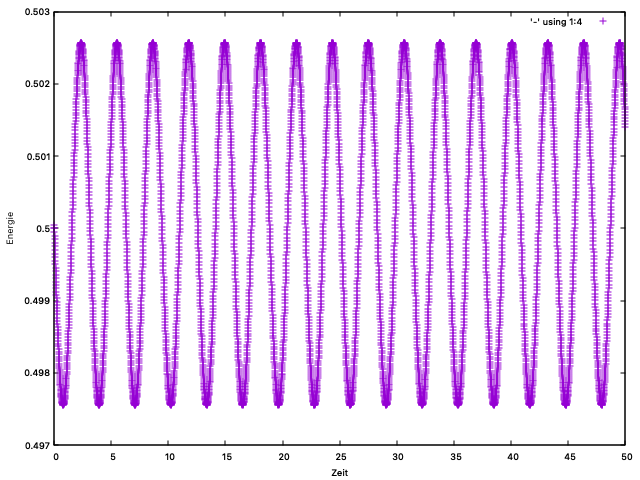
\includegraphics[width=8cm]{Bilddateien/expEulerA1(a)-001h-E.png}
                    \caption{Energiediagramm (man beachte die Skalierung der y-Achse)}
                \end{figure}
                Bis auf minimale Oszillation bleibt diese ebenso konstant.

            \paragraph*{Lösung mit Runge-Kutta (2. Ordnung)}

            \paragraph*{Lösung mit leap-frog}
            
        \subaufgabe{}
            
        \subaufgabe{}

        \subaufgabe{}

        \subaufgabe{}
            

    \newpage
    \subsection*{Hauptcode}
        \lstinputlisting[language=C++]{../src/main.cpp}

    \subsection*{Headerdateien}
        \subsubsection*{Einschrittverfahren}
            \lstinputlisting[language=C++]{../src/header/Einschritt.hpp}

        \subsubsection*{Mehrschrittverfahren}
            \lstinputlisting[language=C++]{../src/header/Mehrschritt.hpp}

        \subsubsection*{Treibende Kräfte}
            \lstinputlisting[language=C++]{../src/header/Funktionsspielereien.hpp}

\end{document}
